\documentclass[conference]{IEEEtran}

\usepackage{graphicx}
\usepackage{subcaption}
\usepackage{amsmath} % assumes amsmath package installed
\usepackage{subcaption}
\usepackage{amssymb}
\usepackage{array}
\usepackage{tikz,circuitikz}
\usetikzlibrary{fit}
\usetikzlibrary{arrows.meta,positioning}
\usepackage{blindtext}
\usepackage{color}
\usepackage{siunitx}
\usepackage{float} % enables [H] float placement
\usepackage{booktabs} % for \toprule, \midrule, \bottomrule
\usepackage[utf8]{inputenc}



\renewcommand{\tablename}{Tabla}

\def\BibTeX{{\rm B\kern-.05em{\sc i\kern-.025em b}\kern-.08em
    T\kern-.1667em\lower.7ex\hbox{E}\kern-.125emX}}


\usepackage{mwe}
\usepackage{fancyhdr}
\fancypagestyle{firststyle}
{
	\fancyhf[C]{\fontsize{8}{10} \selectfont \textit{} }
	\fancyfoot[C]{}
}


\hyphenation{op-tical net-works semi-conduc-tor}


\begin{document}
%
% paper title
% Titles are only capitalized in the first letter.
% Linebreaks \\ can be used within to get better formatting as desired.
% Do not put math or special symbols in the title.
\title{Document title}

\author{\IEEEauthorblockN{1\textsuperscript{st} Given Name Surname}
\IEEEauthorblockA{\textit{dept. name of organization (of Aff.)} \\
\textit{name of organization (of Aff.)}\\
City, Country \\
email address}
\and
\IEEEauthorblockN{2\textsuperscript{nd} Given Name Surname}
\IEEEauthorblockA{\textit{dept. name of organization (of Aff.)} \\
\textit{name of organization (of Aff.)}\\
City, Country \\
email address}
\and
\IEEEauthorblockN{3\textsuperscript{rd} Given Name Surname}
\IEEEauthorblockA{\textit{dept. name of organization (of Aff.)} \\
\textit{name of organization (of Aff.)}\\
City, Country \\
email address}
}


\maketitle

\thispagestyle{firststyle}
\renewcommand{\headrulewidth}{0in}
\pagestyle{empty}


\pagestyle{fancy}
\chead{\fontsize{8}{10} \selectfont \textit{} }
\pagenumbering{gobble}



% As a general rule, do not put math, special symbols or citations
% in the abstract
\begin{abstract}
El documento presenta un análisis de un rectificador semicontrolado trifásico con carga resistiva. Mediante el método de estados asumidos, se determinan las combinaciones válidas de operación,
los rangos de polarización de los SCR y sus ángulos de conducción. Además, se analiza el contenido armónico del voltaje de salida mediante series de Fourier, caracterizando la dependencia de su
componente DC y distorsión armónica con el ángulo de disparo. Los hallazgos analíticos son validados mediante simulaciones en PSIM, confirmando la precisión del modelo teórico.
\end{abstract}


\IEEEpeerreviewmaketitle



\section{Introducción}
Los rectificadores semicontrolados trifásicos representan una configuración clave en aplicaciones de conversión de potencia AC/DC, al ofrecer un compromiso óptimo entre control y simplicidad.
Este trabajo aborda su análisis desde una perspectiva de estados de conducción y calidad espectral de la salida. El método de estados asumidos proporciona un marco riguroso para predecir el
comportamiento de conmutación, mientras que el análisis de Fourier cuantifica el rendimiento en términos de valor medio y distorsión. Mediante las simulaciones en PSIM se verifica la validez
del modelo analítico propuesto. La Fig. \ref{fig:rect}

\begin{figure}[ht]
    \centering
    \begin{circuitikz}[american]
        \ctikzset{
          diodes/scale=0.4, sources/scale=0.5, resistors/scale=0.5, inductors/scale=0.75, capacitors/scale=0.75}

        \draw (-0.75,2.65) to[sV,-*, l={\scriptsize $v_a$},label distance=-2pt,i_>={\scriptsize $i_a$}] (1,2.65)
            node[pos=0.5, right, yshift=  80pt, xshift = 6pt]{\scriptsize $+$}
            node[pos=0.5, left, yshift=80pt, xshift = 1pt]{\scriptsize $-$};
        \draw (-0.75,2.00) to[sV, l={\scriptsize $v_b$},label distance=-2pt,i_>={\scriptsize $i_b$}] (1,2.00)
            node[pos=0.5, right, yshift=  61pt, xshift = 6pt]{\scriptsize $+$}
            node[pos=0.5, left, yshift=61pt, xshift = 1pt]{\scriptsize $-$};
        \draw (-0.75,1.35) to[sV, l={\scriptsize $v_c$},label distance=-2pt,i_>={\scriptsize $i_c$}] (1,1.35)
            node[pos=0.5, right, yshift=42pt, xshift = 6pt]{\scriptsize $+$}
            node[pos=0.5, left, yshift=42pt, xshift = 1pt]{\scriptsize $-$};

        \draw (1,0)   to[Ty*, l={\scriptsize $T_4$}, label distance=-10mm] (1,1.35)
                  to[short] (1,2.65)
                  to[Ty*, l={\scriptsize $T_1$}, label distance=-10mm] (1,4);

        \draw (1.75,0) to[Ty*, l={\scriptsize $T_6$}, label distance=-10mm] (1.75,1.35)
                  to[short] (1.75,2.65)
                  to[Ty*, l={\scriptsize $T_3$}, label distance=-10mm] (1.75,4);

        \draw (2.5,0)   to[Ty*, l={\scriptsize $T_2$}, label distance=-10mm] (2.5,1.35)
                  to[short] (2.5,2.65)
                  to[Ty*, l={\scriptsize $T_5$}, label distance=-10mm] (2.5,4);

        \draw (4,0) to[R, l={\scriptsize $R$}, v_<={\scriptsize $v_R$}, f<^={\scriptsize $i_R$}] (4,4);
        \draw (1,4) -- (2,4) to[short, i>^={\scriptsize $i_{oi}$}] (4,4);
        \draw (1,0) to[short] (4,0);
        \draw (-0.75,1.35) -- (-0.75,2.65);
        \draw (-0.75,2) node[left]{\scriptsize $n$};
        \draw (1,1.35) to[short,-*] (2.5,1.35);
        \draw (1,2) to[short,-*] (1.75,2);
        \draw (2.5,0) -- (2.5,4)
            node[pos=0.5, right]{\scriptsize $v_{oi}$}
            node[pos=0.9, right]{\scriptsize $+$}
            node[pos=0.1, right]{\scriptsize $-$};

	\end{circuitikz}
	\caption{Rectificador semicontrolado trifásico}
	\label{fig:rect}
\end{figure}

Lo voltajes de línea a nueutro se definen como:
\begin{equation*}
	\begin{aligned}
		v_a(t) &= V_{max}\sin(\omega t) \\
		v_b(t) &= V_{max}\sin(\omega t - 120^\circ) \\
		v_c(t) &= V_{max}\sin(\omega t + 120^\circ)
	\end{aligned}
\end{equation*}

\section{Estados asumidos}

	En un instante dado las tres tensiones de fase $v_a,v_b,v_c$ se ordenan por su valor instantáneo; con SCR ideales y sin solape, siempre conducen dos dispositivos: el superior de la fase con mayor potencial y el inferior de la fase con menor potencial, de modo que el voltaje de salida es siempre un línea–a–línea $v_{oi}(t)=v_{\max}(t)-v_{\min}(t)$. Se considera además el estado sin conducción $S_0$ cuando aún no se ha aplicado el pulso de compuerta (ángulo $\alpha$) o la red no supera el umbral de disparo. Así, los siete estados son: 
	
	\begin{itemize}
		\item $S_0$: ningún SCR conduce, $v_{oi}=0$.
		\item $S_1$ si $v_a\ge v_b\ge v_c$, $T_1$ y $T_6$ (ON), $v_{oi}=v_a-v_b\equiv v_{ab}$.
		\item $S_2$ si $v_a\ge v_c\ge v_b$, $T_1$ y $T_2$ (ON), $v_{oi}=v_a-v_c\equiv v_{ac}$.
		\item $S_3$ si $v_b\ge v_a\ge v_c$, $T_3$ y $T_4$ (ON), $v_{oi}=v_b-v_a\equiv v_{ba}$.
		\item $S_4$ si $v_b\ge v_c\ge v_a$, $T_3$ y $T_2$ (ON), $v_{oi}=v_b-v_c\equiv v_{bc}$.
		\item $S_5$ si $v_c\ge v_a\ge v_b$, $T_5$ y $T_4$ (ON), $v_{oi}=v_c-v_a\equiv v_{ca}$.
		\item $S_6$ si $v_c\ge v_b\ge v_a$, $T_5$ y $T_6$ (ON), $v_{oi}=v_c-v_b\equiv v_{cb}$. 
	\end{itemize}

	Las transiciones entre estados ocurren cuando dos tensiones de fase se igualan (cruces $v_a=v_b$, $v_b=v_c$ o $v_c=v_a$), lo que en el caso senoidal balanceado sucede cada $60^\circ$ eléctricos; el inicio efectivo de cada estado conductor queda retrasado por el ángulo de disparo $\alpha$. Dado que la carga es estrictamente resistiva, no hay almacenamiento de energía ni memoria de estado: la corriente sigue instantáneamente a la tensión en cada tramo y vale simplemente
		\begin{equation*}
			i(t)=\frac{v_{oi}(t)}{R},
		\end{equation*}
	anulándose exactamente en los instantes de cambio de par, por lo que el apagado de los SCR es natural en cada frontera de \(60^\circ\).

% (p. ej., \(T_1\) a \(\omega t=\tfrac{\pi}{6}+\alpha\), \(T_2\) a \(\tfrac{\pi}{2}+\alpha\), etc.)

\begin{table}[h!]
	\centering
	\small
	\begin{tabular}{@{}cc@{}}
		\toprule
		Estado & Intervalo (grados) \\ \midrule
	    $S_{1}$ & $[30^\circ+\alpha,\;90^\circ+\alpha]$ \\
		$S_{2}$ & $[90^\circ+\alpha,\;150^\circ+\alpha]$ \\
		$S_{3}$ & $[150^\circ+\alpha,\;210^\circ+\alpha]$ \\
		$S_{4}$ & $[210^\circ+\alpha,\;270^\circ+\alpha]$ \\
		$S_{5}$ & $[270^\circ+\alpha,\;330^\circ+\alpha]$ \\
		$S_{6}$ & $[330^\circ+\alpha,\;390^\circ+\alpha]$ \\ \bottomrule
	\end{tabular}
	\caption{Intervalos de los estados asumidos.}
	
	\label{tab:estados_grados}
\end{table}

En cada intervalo de $60^\circ$ la secuencia de fases (desfasadas $120^\circ$) produce una fase 
con mayor potencial y otra con menor potencial; el par de tiristores del sector conecta dicha fase 
máxima con la mínima, por lo que $v_{oi}$ en ese tramo es la diferencia línea-a-línea entre ellas. 
El ángulo de disparo $\alpha$ no altera el orden relativo de las fases: simplemente \emph{desplaza} el inicio de cada sector (p. ej. $S_{1}$ comienza en $30^\circ+\alpha$, 
$S_{2}$ en $90^\circ+\alpha$, etc.). En un modelo ideal por tramos cada sector dura $60^\circ$.

El voltaje promedio ($V_{cd}$) en los terminales de la carga $R$ se obtiene según la siguiente ecuación, donde $V_m$ es el voltaje máximo.
\begin{align*}	
    V_{cd} &= \frac{3\sqrt{3}\,V_m}{\pi} \cos\alpha	
\end{align*}

Mientras el voltaje $rms$ ($V_{\text{rms}}$) se obtiene como:
\begin{align*}	
    V_{\text{rms}} &= \sqrt{3}V_m\sqrt{\frac{1}{2} + \frac{3\sqrt{3}}{4\pi} \cos 2\alpha}
\end{align*}


\section{Simulación en PSIM}

%La Fig.\ref{fig:rec_trifasico} muestra el comportamiento del voltaje en la resistencia $v_r$
%para el rectificador trifásico.

%\begin{figure}[H]
%\centering
%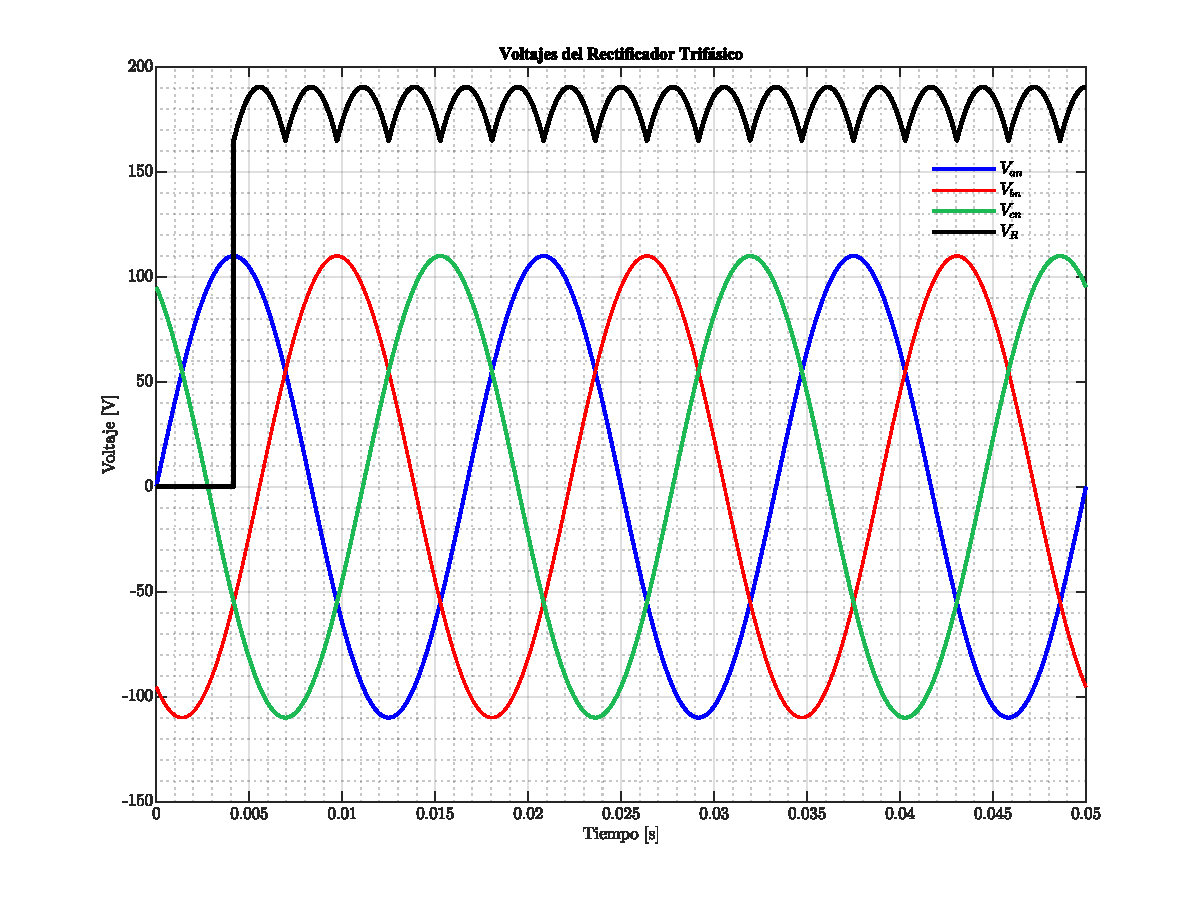
\includegraphics[width=0.75\linewidth]{Fig/Rectificador_trifasico.pdf}
%\caption{Comportamiento de $v_R$}
%\label{fig:rec_trifasico}
%\end{figure}

Para obtener este resultado se ajusto el ángulo de disparo de cada tiristor según la Tabla \ref{tab:angulos_disparo}

\begin{table}[h!]
	\centering
	\small
	\begin{tabular}{@{}cc@{}}
		\toprule
		Estado & Intervalo (grados) \\ \midrule
	    $T_{1}$ & $[30^\circ- 150^\circ]$ \\
		$T_{2}$ & $[90^\circ- 210^\circ]$ \\
		$T_{3}$ & $[150^\circ-270^\circ]$ \\
		$T_{4}$ & $[210^\circ-330^\circ]$ \\
		$T_{5}$ & $[270^\circ-390^\circ]$ \\
		$T_{6}$ & $[330^\circ-450^\circ]$ \\ \bottomrule
	\end{tabular}
	\caption{Ángulos de disparo para cada tiristor}
	\label{tab:angulos_disparo}
\end{table}


\begin{figure}[ht]
	\centering
	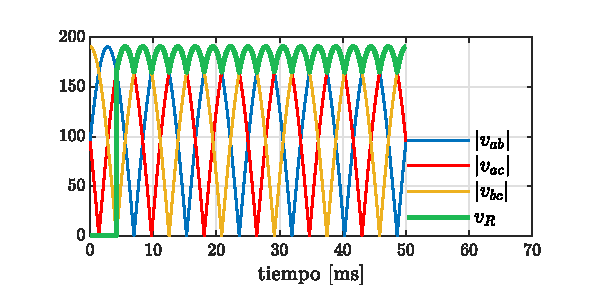
\includegraphics[scale=1]{Fig/volt_lin_R.eps}
	\caption{Voltaje de salida del rectificador trifásico}
	\label{fig:v_oi_cero}
\end{figure}

\begin{figure}[ht]
	\centering
	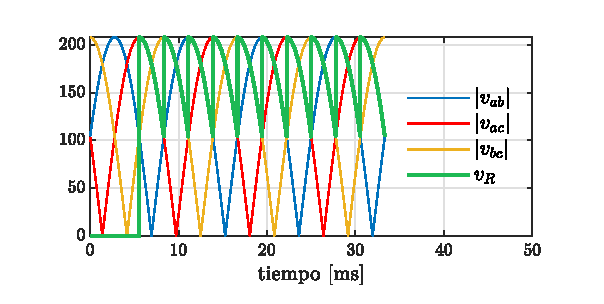
\includegraphics[scale=1]{Fig/volt_lin_R30.eps}
	\caption{Voltaje de salida del rectificador trifásico con $\alpha=30^\circ$}
	\label{fig:v_oi_tre}
\end{figure}

\section{Analis de Fourier de la señal de Salida $v_{oi}$}
El voltaje de salida \(v_o(\omega t)\) puede expresarse mediante su serie de Fourier:

\[
v_o(\omega t) = a_0 + \sum_{n=1}^{\infty} \left[a_n \cos(n\omega t) + b_n \sin(n\omega t)\right]
\]
los coeficientes son:
\[
a_0 = V_{cd}
\]
\[
a_n = \frac{6}{\pi} \sqrt{3} V_m \int_{\frac{\pi}{6} + \alpha}^{\frac{\pi}{2} + \alpha} \sin\left(\omega t + \frac{\pi}{6}\right) \cos(n\omega t)  d(\omega t)
\]

\[
b_n = \frac{6}{\pi} \sqrt{3} V_m \int_{\frac{\pi}{6} + \alpha}^{\frac{\pi}{2} + \alpha} \sin\left(\omega t + \frac{\pi}{6}\right) \sin(n\omega t)  d(\omega t)
\]
Los coeficientes $a_{n}$ y $b_{n}$ representan los armonicos de la señal de salida. 
Los armónicos dominantes en el voltaje de salida son múltiplos de 6 (\(n = 6, 12, 18, \ldots\)) 
debido a la simetria de la señal, ya que la conmutacion de los SCR ocurre cada \(60^\circ\) 
(\(\pi/3\) radianes). La señal se repite cada \(\pi/3\) radianes, por lo que la frecuencia 
fundamental es \(6f\).  Al aumentar \(\alpha\), los armónicos aumentan debido que los coeficientes 
 $a_{n}$ y $b_{n}$ presentan una relacion sinosoidal proporcional a \(\alpha\), en \(0^\circ\) los armonicos 
 son minimos, en \(90^\circ\) se presenta el mayot contenido armonico y en \(>90^\circ\) el contenido armonico
 disminuye. 


\section{Conclusiones}
El método de estados asumidos es una herramienta eficaz para identificar las configuraciones válidas en el circuito, definiendo los límites de polarización directa/inversa
y los rangos de ángulo de disparo para los SCR.

El análisis de series de Fourier estableció una relación directa y cuantificable entre $\alpha$ y el espectro de salida: el valor DC decrece inversamente con $\alpha$,
mientras que el $THD$ se modifica sustancialmente.

Las simulaciones en PSIM corroboraron los modelos analíticos, verificando las formas de onda de conducción y los espectros armónicos obtenidos teóricamente.

\begin{thebibliography}{plain}
\bibitem{b1} G. Eason, B. Noble, and I. N. Sneddon, ``On certain integrals of Lipschitz-Hankel type involving products of Bessel functions,'' Phil. Trans. Roy. Soc. London, vol. A247, pp. 529--551, April 1955.
\bibitem{b2} J. Clerk Maxwell, A Treatise on Electricity and Magnetism, 3rd ed., vol. 2. Oxford: Clarendon, 1892, pp.68--73.
\bibitem{b3} I. S. Jacobs and C. P. Bean, ``Fine particles, thin films and exchange anisotropy,'' in Magnetism, vol. III, G. T. Rado and H. Suhl, Eds. New York: Academic, 1963, pp. 271--350.
\bibitem{b4} K. Elissa, ``Title of paper if known,'' unpublished.
\bibitem{b5} R. Nicole, ``Title of paper with only first word capitalized,'' J. Name Stand. Abbrev., in press.
\bibitem{b6} Y. Yorozu, M. Hirano, K. Oka, and Y. Tagawa, ``Electron spectroscopy studies on magneto-optical media and plastic substrate interf	ace,'' IEEE Transl. J. Magn. Japan, vol. 2, pp. 740--741, August 1987 [Digests 9th Annual Conf. Magnetics Japan, p. 301, 1982].
\bibitem{b7} M. Young, The Technical Writer's Handbook. Mill Valley, CA: University Science, 1989.
\end{thebibliography}


\end{document}